\documentclass[
	%sans,			% use sans-serif font
	%serif,			% use serif-font
	%mathsans,		% set mathtext to sans-serif
	%mathserif,		% set mathtext to serif
	%10pt,
	10pt,
	%12pt,
	t		% add text at the top border of slide
	%slidescentered,% center text on slide
	%draft,			% compile as draft version
	%handout,		% create handout file
	%notes,			% include nodes in slides
	%compress		% compress navigation bar
]{beamer}


\usetheme{lmtslides}
\usepackage{eso-pic}
%\usepackage[pdftex]{color}
\usepackage{times}
\usepackage[latin1]{inputenc}
%\usepackage[T1]{fontenc}
\usepackage[amssymb]{SIunits}
\usepackage{amsmath,amssymb}
\usepackage{eurosym}
\usepackage{booktabs}
\usepackage{colortbl}
\usepackage{url}
\usepackage{animate}
\usepackage{graphics}

\graphicspath{{figures/}}

% SET LANGUAGE HERE! (Babel is already included and setup by this call.)
%\setlang{de}		% <- GERMAN
\setlang{en}		% <- ENGLISH

% MODIFY THESE ACCORDINGLY! ---
\title{Parallel Mesh Simplification with Adaptive Thresholding Based on Quadric Error Metrics}
\subtitle{Interdisciplinary project}
\type{Sf} % (M/B/D/S)(f/m): (Master/Bachelor/Diplom/Studienarbeit)(final/midterm)
\author{Wojciech Zielonka}
\email{wojciech.zielonka@tum.de}
\advisor{Prof. Dr.-Ing. Eckehard Steinbach}
\emailAdvisor{eckehard.steinbach@tum.de}
\date{\today}
%------------------------------


%%%%%%%%%%%%%%%%%%%%%%%%%%
\begin{document}

\AddToShipoutPicture{\TitlePicture}
\maketitle
\ClearShipoutPicture
\AddToShipoutPicture{\BackgroundPicture}

\section{Get from}
\begin{frame}
\frametitle{How to get from this mesh?}
\begin{figure}[ht]
	\centering
    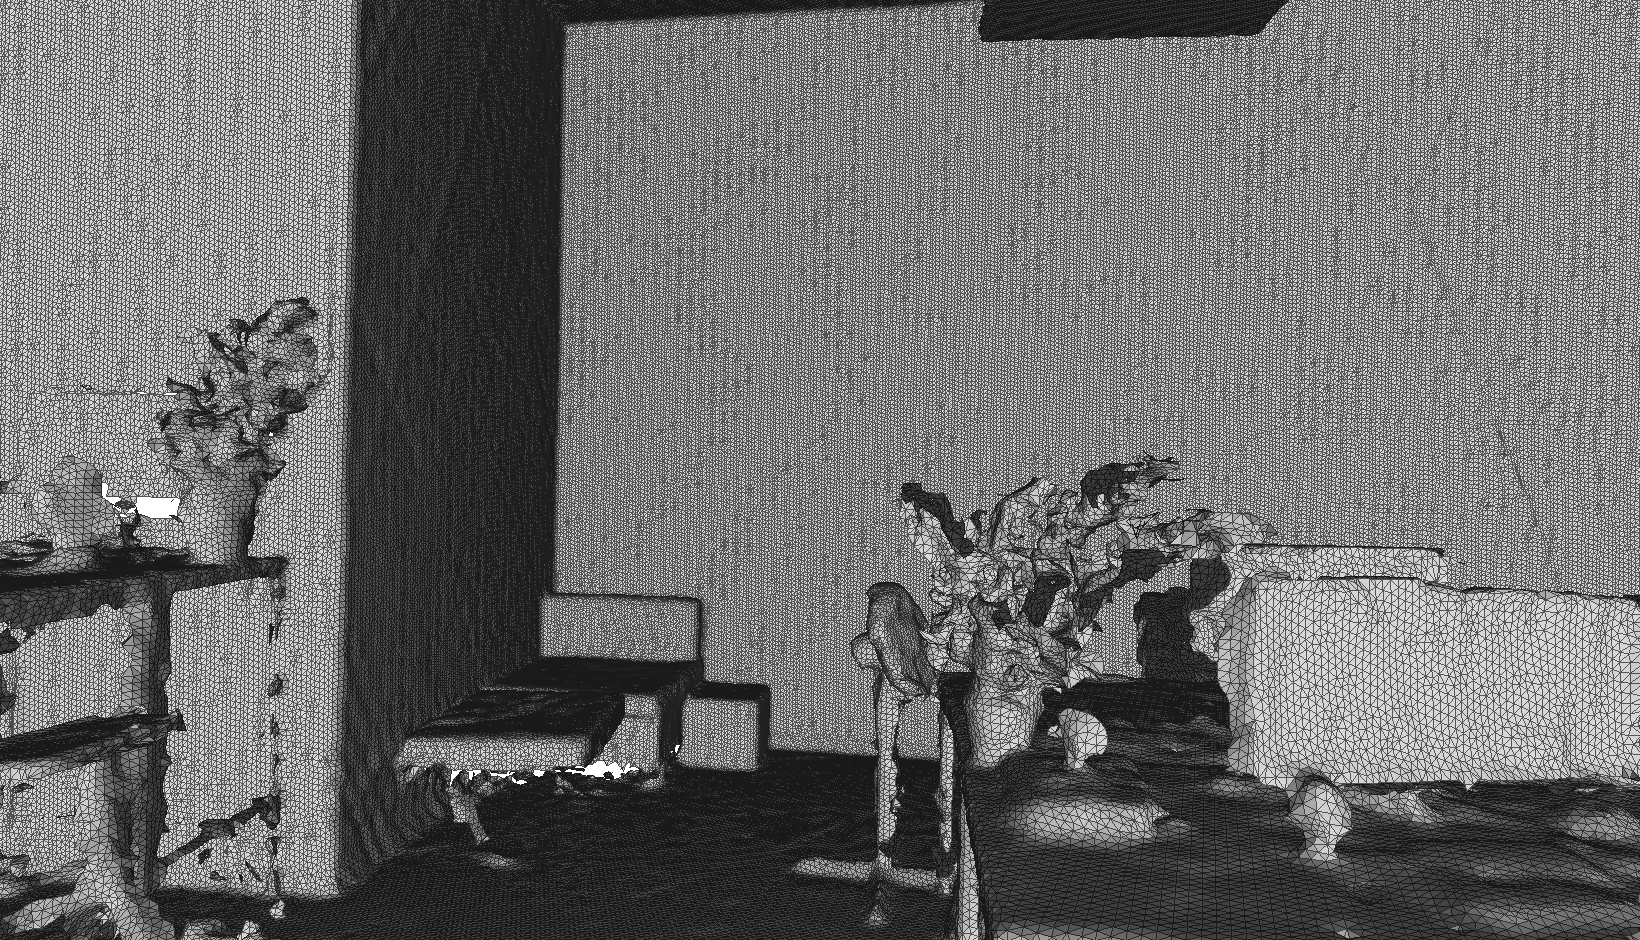
\includegraphics[width=1\textwidth]{from}
\end{figure}
\end{frame}

\section{To}
\begin{frame}
\frametitle{To this mesh?}
\begin{figure}[ht]
	\centering
    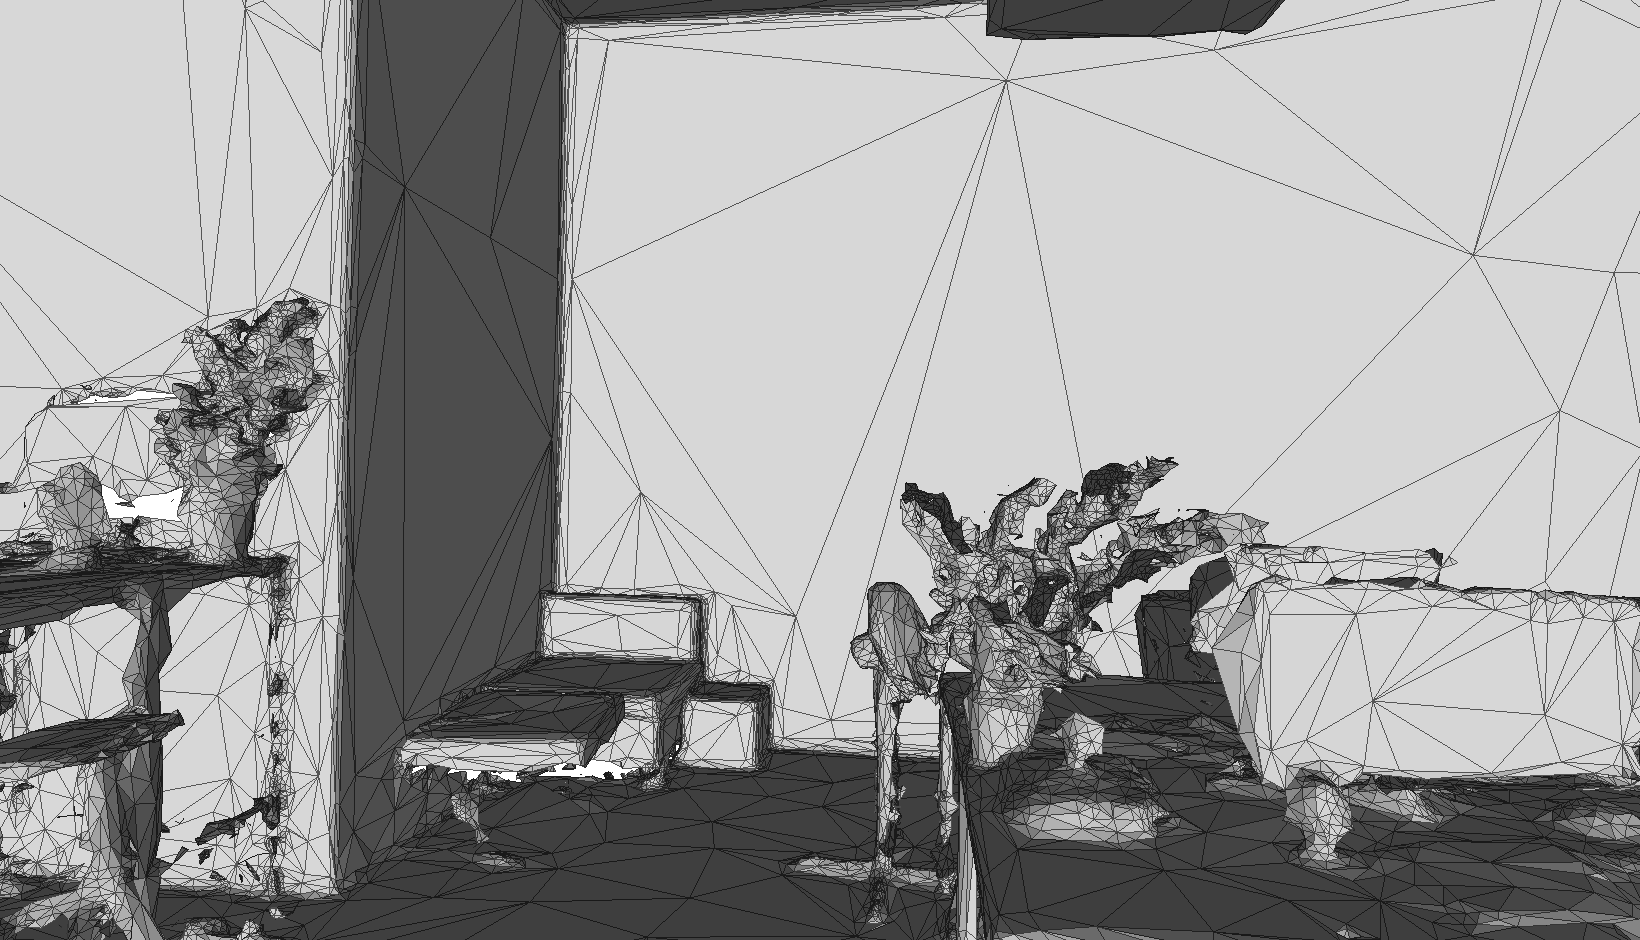
\includegraphics[width=1\textwidth]{to}
\end{figure}
\end{frame}

\section{Assumptions}
\begin{frame}
\frametitle{Assumptions}
\begin{enumerate}
\centering
\item Simplify mostly planar surface.
\item Preserve complex shapes as much as possible.
\item Use a parallel framework.
\end{enumerate}
\end{frame}

\section{What is a decimation}
\begin{frame}
\frametitle{What is a decimation?}
\begin{figure}[ht]
\centering
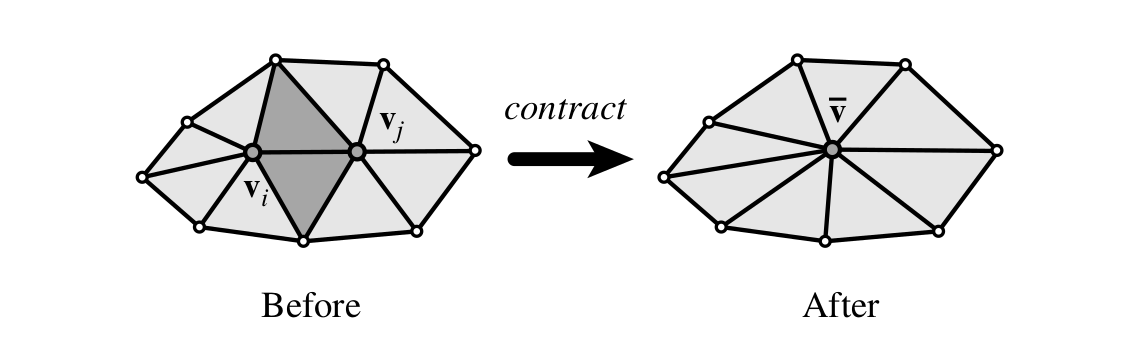
\includegraphics[width=1\textwidth]{edge_contraction}
\end{figure}
\end{frame}

\section{How to find an edge}
\begin{frame}
\frametitle{How to select edges?}
\centering
\begin{enumerate}
\item Select a set of candidate vertex pairs $(\mathbf{v_i}, \mathbf{v_j})$.
\item Allocate a quadric $Q_i$ for each vertex $\mathbf{v_i}$.
\item For each face compute a quadric $Q_i$. Add this quadric to the vertex quadrics $Q_i, Q_k, Q_l$ and optionally weight it appropriately.
\item For each candidate pair $(\mathbf{v_i}, \mathbf{v_j})$:
\begin{enumerate}
\item Compute $Q = Q_i + Q_j$.
\item Select a target position $\mathbf{\bar{v}}$.
\item Apply consistency checks and penalties.
\item Place pair in heap keys on cost $Q(\mathbf{\bar{v}})$
\end{enumerate}
\item Repeat until the desired approximation is reached:
\begin{enumerate}
\item Remove the pair $(\mathbf{v_i}, \mathbf{v_j})$ of least cost from the heap.
\item Preform contraction $(\mathbf{v_i}, \mathbf{v_j})\rightarrow\bar{\mathbf{v}}$
\item Set $Q_i = Q_i + Q_j$.
\item For each remaining pair $(\mathbf{v_i}, \mathbf{v_j})$, compute target position and cost as in step 4; update heap.
\end{enumerate}
\end{enumerate}
\end{frame}

\section{Quadric}
\begin{frame}
\frametitle{What is Quadric?}
\centering
$\mathbf{n}^T\mathbf{v}+d=0$\\ normal $\mathbf{n} = [a\;b\;c]^T$\\ $d$ is a scalar constant\\ $\mathbf{v} = [x\;y\;z]^T$ is a point in $3D$ space.
\\
\begin{align}
D^2(\mathbf{v}) &= (\mathbf{n}^T\mathbf{v}+d)^2 = (\mathbf{v}^T(\mathbf{n}\mathbf{n}^T)\mathbf{v}+2(d\mathbf{n})^T\mathbf{v}+d^2)\\
Q(\mathbf{v}) &= \mathbf{v}^T\mathbf{A}\mathbf{v} + 2\mathbf{b}^T\mathbf{v} + c\\
Q(\mathbf{v}) &= D^2(\mathbf{v})
\end{align}
\end{frame}

\section{Quadric accumulation}
\begin{frame}
\frametitle{Quadric accumulation}
\centering
\begin{enumerate}
\item Allocate a quadric $Q_i$ for each vertex $\mathbf{v_i}$.
\item For each face compute a quadric $Q_f$. Add this quadric to the vertex quadrics $Q_i, Q_k, Q_l$ and optionally weight it appropriately.
\end{enumerate}
\end{frame}

\section{Create edges}
\begin{frame}
\frametitle{Create edges}
\centering
\begin{enumerate}
\item For each candidate pair $(\mathbf{v_i}, \mathbf{v_j})$:
\begin{enumerate}
\item Compute $Q = Q_i + Q_j$.
\item Select a target position $\mathbf{\bar{v}}$.
\item Apply consistency checks and penalties.
\item Place pair in heap keys on cost $Q(\mathbf{\bar{v}})$
\end{enumerate}
\end{enumerate}
\end{frame}

\section{Heap iterations}
\begin{frame}
\frametitle{Heap iterations}
\centering
\begin{enumerate}
\item Repeat until the desired approximation is reached:
\begin{enumerate}
\item Remove the pair $(\mathbf{v_i}, \mathbf{v_j})$ of least cost from the heap.
\item Preform contraction $(\mathbf{v_i}, \mathbf{v_j})\rightarrow\bar{\mathbf{v}}$
\item Set $Q_i = Q_i + Q_j$.
\item For each remaining pair $(\mathbf{v_i}, \mathbf{v_j})$, compute target position and cost as in step 4; update heap.
\end{enumerate}
\end{enumerate}
\end{frame}

\section{Extended version with color and normals}
\begin{frame}
\frametitle{Extended version with color and normals}
\centering

\end{frame}


\section{Adaptive thresholding}
\begin{frame}
\frametitle{Adaptive thresholding}
\centering

\end{frame}

\section{How make it faster}
\begin{frame}
\frametitle{How to make it faster?}
\centering

\end{frame}

\section{Iterations}
\begin{frame}
\begin{center}
\animategraphics[autoplay,loop, width=10cm]{0.1}{snapshot}{1}{5}
\end{center}
\end{frame}

\section{Vortragsfolien}
\begin{frame}
\frametitle{Vortragsfolien}
\end{frame}

\end{document}
